% Chapter Template

\chapter{Results and Discussion}
\label{Chapter5}

As briefly mentioned towards the end of Section \refsec:reachableSphere}, the code base used in this project, and particularly the retargeting part implementing the whole Egocentric Coordinate formalism, is problematic. Although well formated and making use of carefully chosen variable names, the code is intrinsically complex and has sadly not been well documented nor commented.

This unfortunately forced us to reconsider the schedule for this project, and prevented us from performing the experiment described in Chapter \ref{Chapter4}. Luckily, we will be able to continue this project in the next six months thanks to a project grant by the Hassler Foundation, hence making it possible to run the experiment and publish its results in a subsequent report.

The remainder of this chapter therefore does not describe the results of the experiment itself, but what we have been able to achieve software-wise in terms of distortion and experiment implementation.

\section{Distortion}

A few examples of distortion and the resulting poses have already been shown on Figures \ref{fig:armExamples} and \ref{fig:divergence}. We propose here a more detailed summary of our results and a discussion of them.


\begin{figure}[h]
    \centering
    \begin{subfigure}[b]{.3\textwidth}
        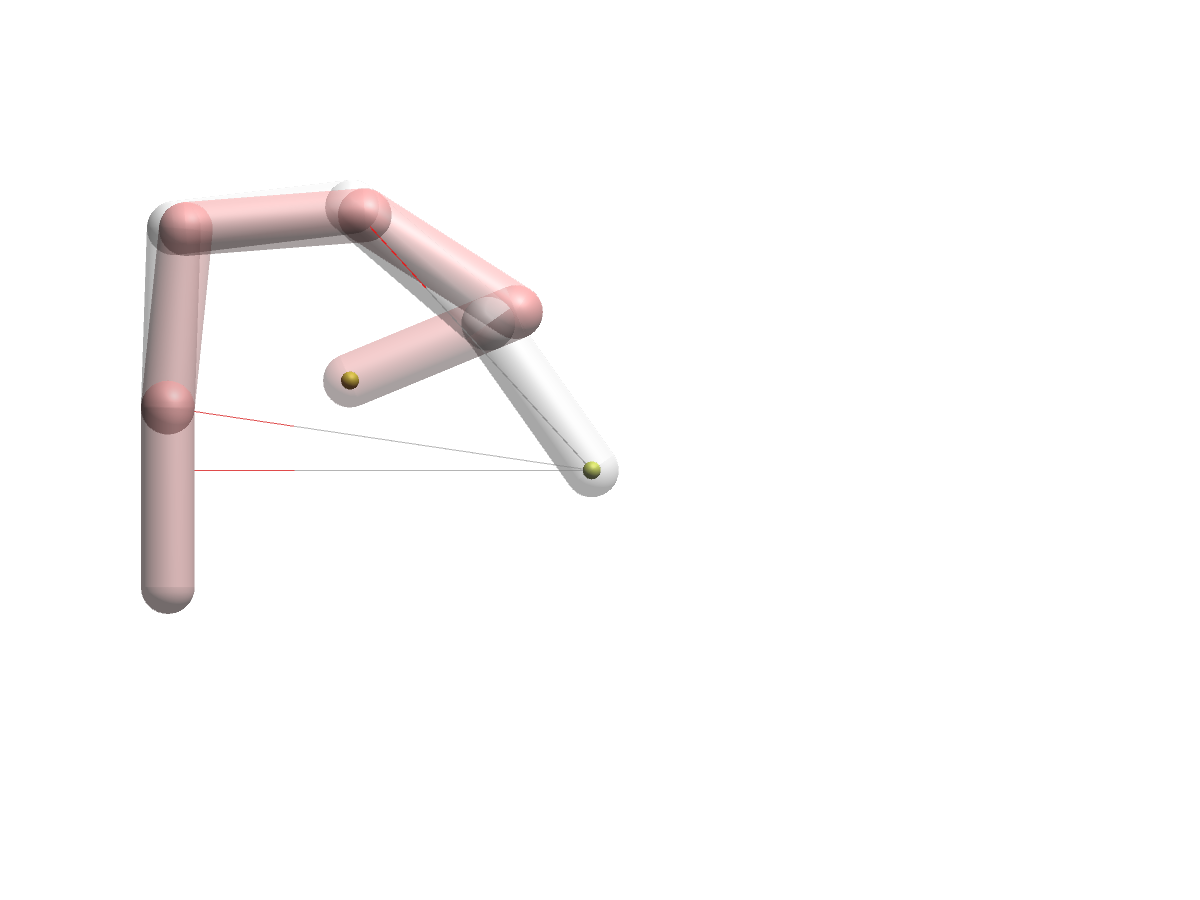
\includegraphics[width=\textwidth]{Figures/distortions/distortions-6.png}
        \caption{$\gamma = -6$}
    \end{subfigure}
    ~
    \begin{subfigure}[b]{.3\textwidth}
        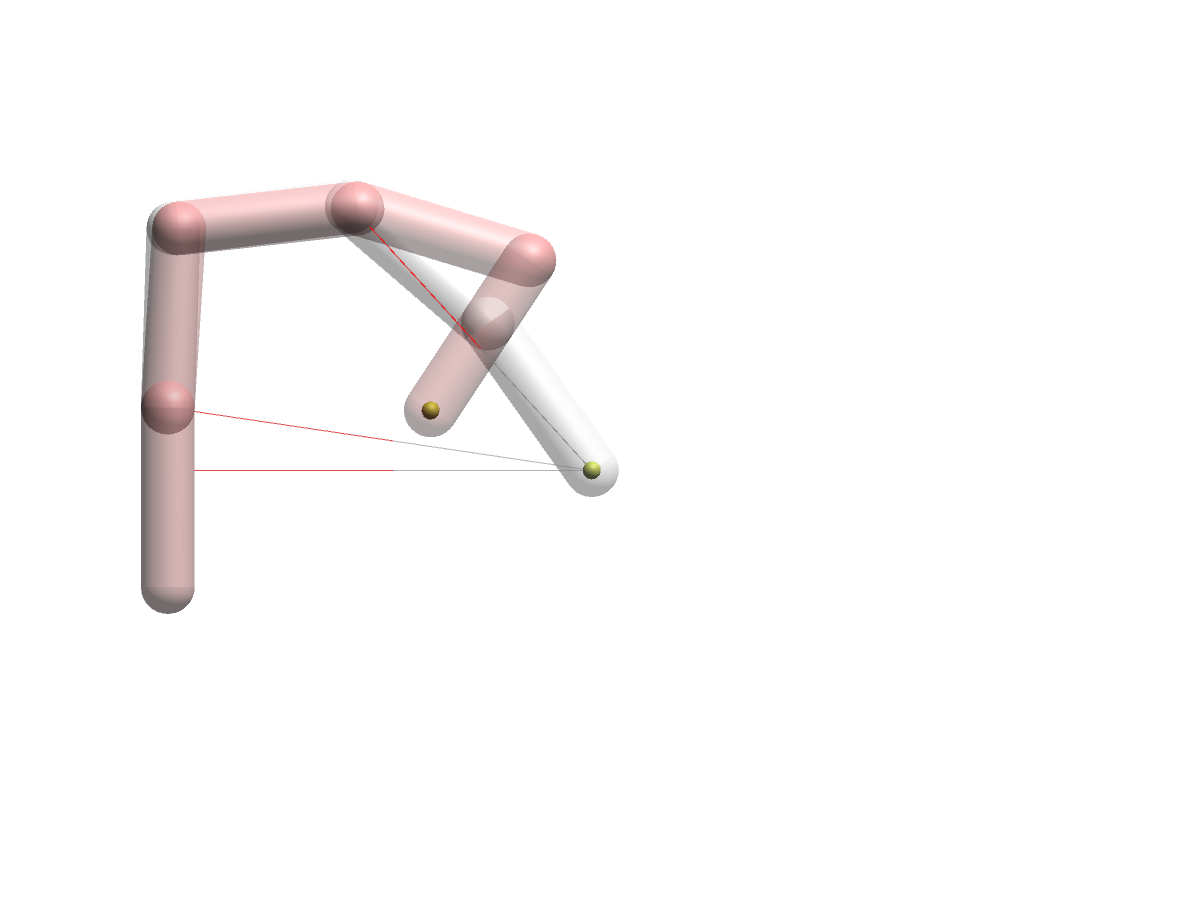
\includegraphics[width=\textwidth]{Figures/distortions/distortions-3.png}
        \caption{$\gamma = -3$}
    \end{subfigure}
    ~
    \begin{subfigure}[b]{.3\textwidth}
        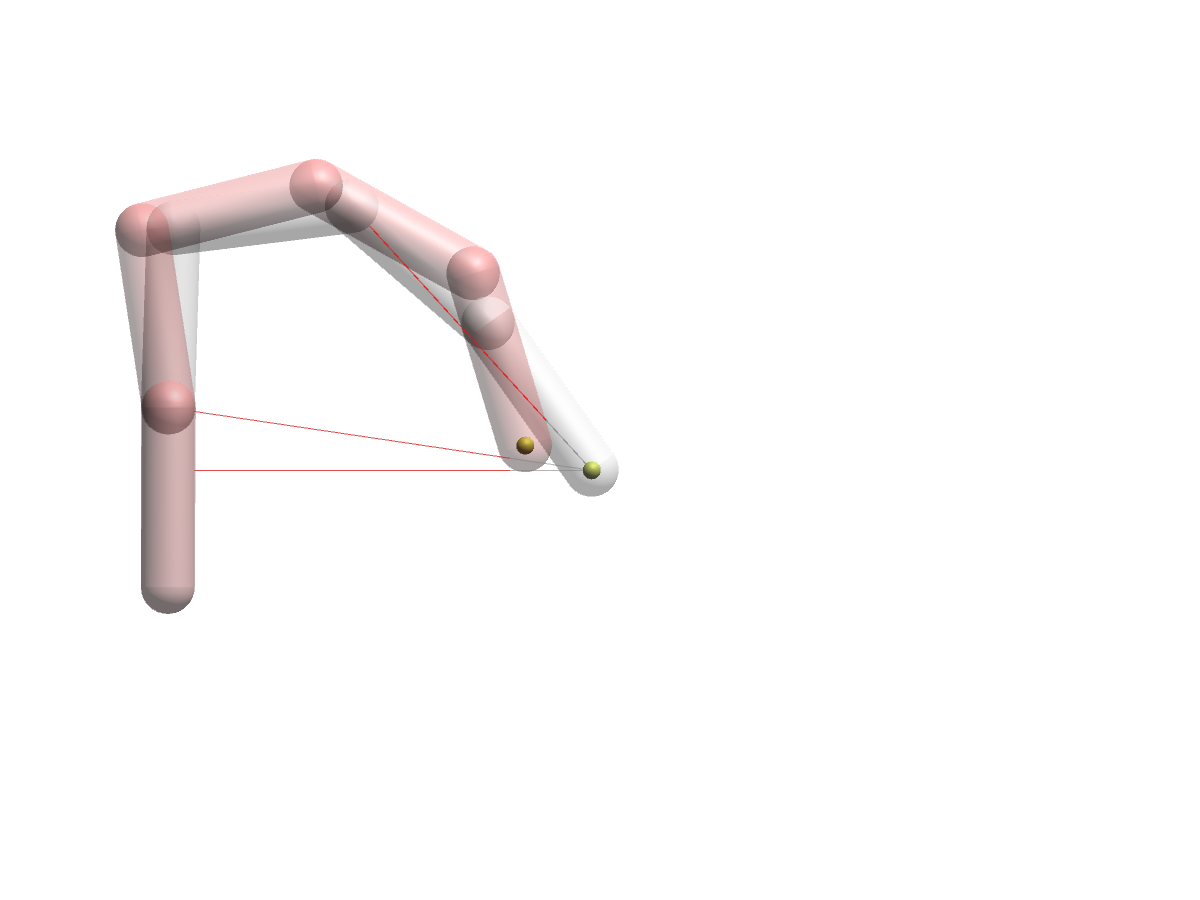
\includegraphics[width=\textwidth]{Figures/distortions/distortions-1.png}
        \caption{$\gamma = -1$}
    \end{subfigure}
    
    
    \begin{subfigure}[b]{.3\textwidth}
        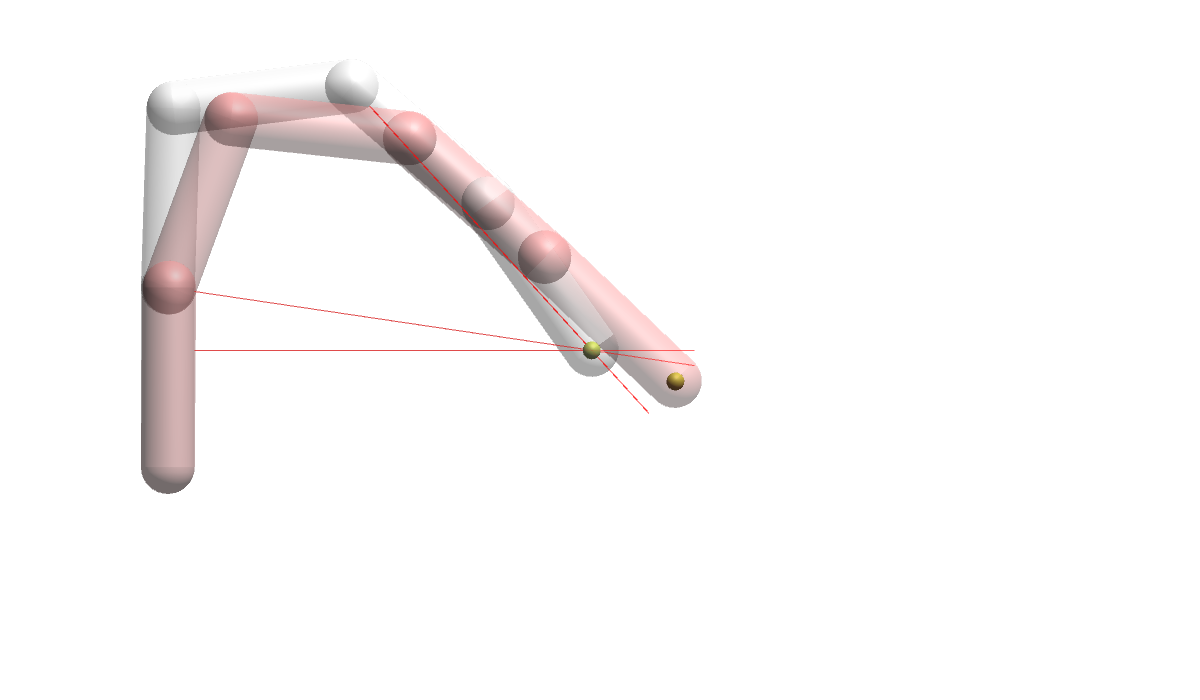
\includegraphics[width=\textwidth]{Figures/distortions/distortions1.png}
        \caption{$\gamma = 1$}
    \end{subfigure}
    ~
    \begin{subfigure}[b]{.3\textwidth}
        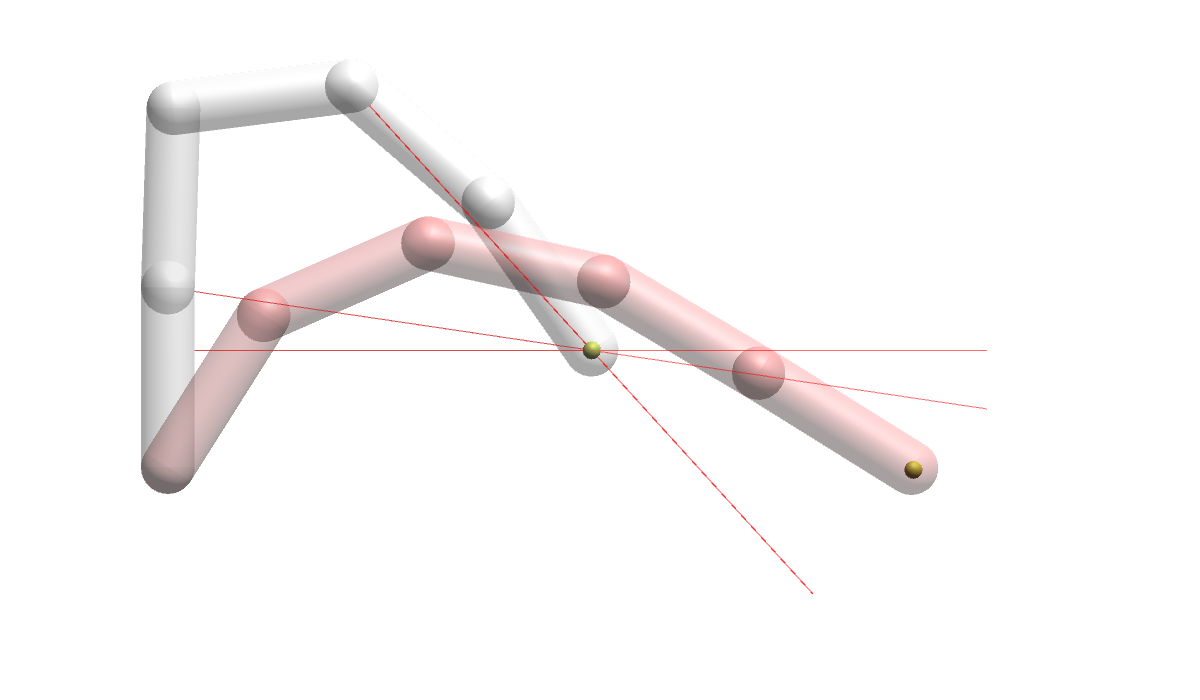
\includegraphics[width=\textwidth]{Figures/distortions/distortions3.png}
        \caption{$\gamma = 3$}
    \end{subfigure}
    ~
    \begin{subfigure}[b]{.3\textwidth}
        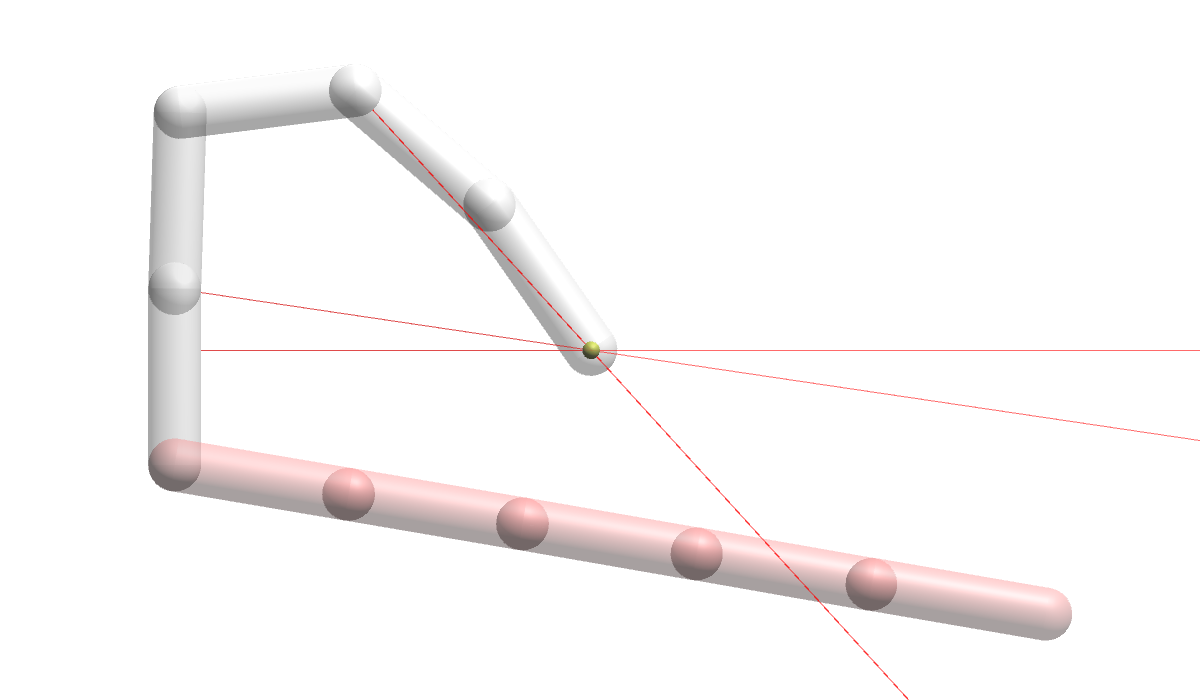
\includegraphics[width=\textwidth]{Figures/distortions/distortions6.png}
        \caption{$\gamma = 6$}
        \label{subfig:gamma6}
    \end{subfigure}
        
    \caption{An example of distorted poses. As always, the captured arms are in gray, the distorted ones in red, and the red and gray lines respectively represent the distorted and original Egocentric coordinates.}
    \label{fig:distortionExamples}
\end{figure}

As one can observe on Figure \ref{fig:distortionExamples}, the distortion works the way it is expected to. As a reminder, a gain of $\pm\SI{6}{\decibel}$ corresponds to a movement whose amplitude is respectively multiplied by $3.981$ and $0.251$, which means it is changed almost fourfold in each direction with respect to a non distorted one. A value of $\gamma = \pm\SI{1}{\decibel}$ similarly modifies a movement by $1.259$ or $0.794$.

The behavior of the arm in Figure \ref{subfig:gamma6} is precisely the one we proposed to avoid using the reachable sphere described in Section \ref{sec:reachableSphere} but we do not report on it here because, as previously justified, we did not implement it in our experiment.

An interactive web application where one may play with both the real arm position and the gain of the distortion, as well as toggling the presence or not of the reachable sphere, is available at \url{https://sidneybovet.github.io/amplified-embodiment/}. The reader is encouraged to play with the IK chain in order to get a better feeling for how the distortion works, especially how it behaves near the skin.

In order to better understand how such a distortion applies to a captured motion, Figure \ref{fig:realMocapDistortion} shows a subject performing a reaching motion towards the air target. The virtual hand is at the same position on all three pictures, but as one may observe, the subject has his hand at different positions. This is due to the fact that in one case (higher hand position) no distortion was applied, while the other (lower hand position) sees a distortion of \SI{3}{\decibel}. The central image shows the superimposition of the two poses in order to better see the position discrepancy.

\begin{figure}[h]
    \centering
    \begin{subfigure}[b]{.3\textwidth}
        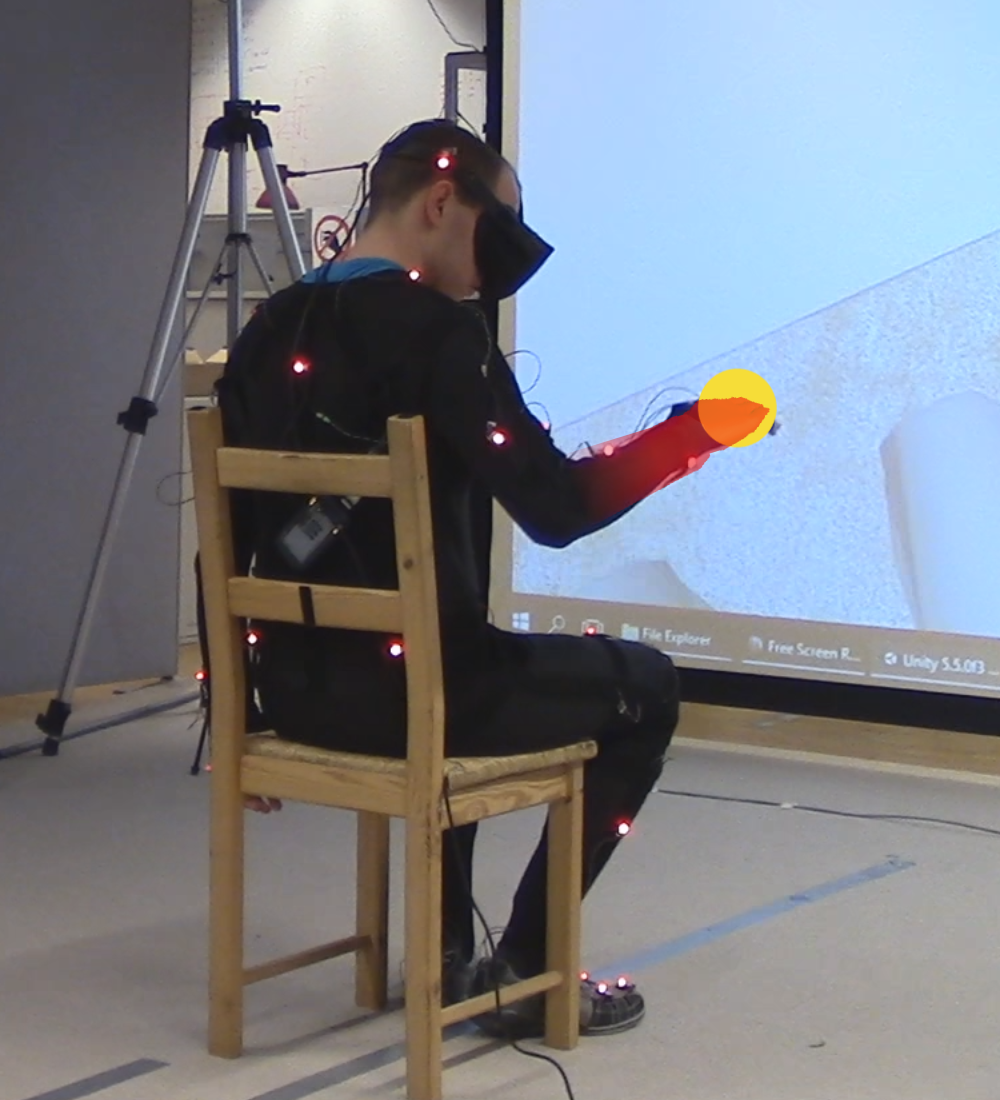
\includegraphics[width=\textwidth]{Figures/handPositionTargetNoDist.png}
    \end{subfigure}
    ~
    \begin{subfigure}[b]{.3\textwidth}
        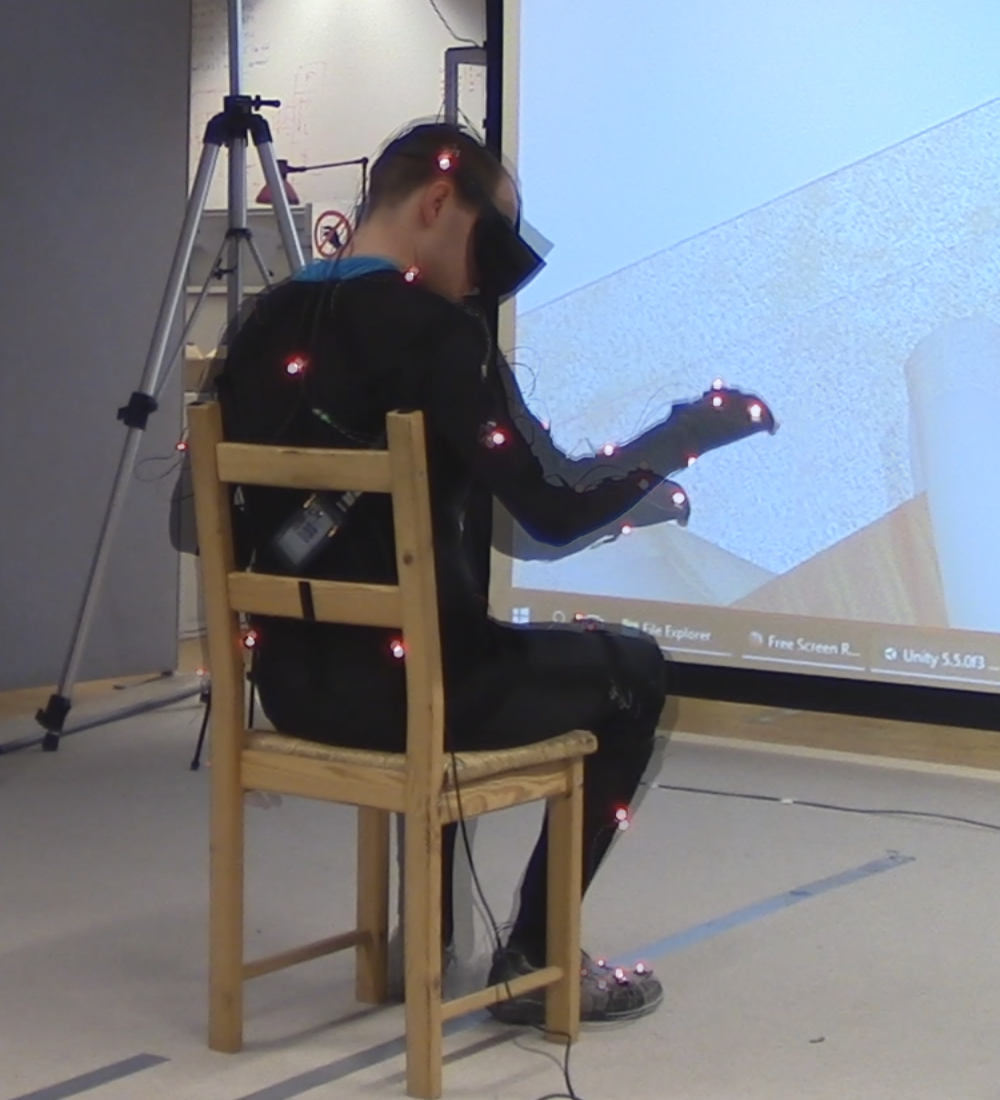
\includegraphics[width=\textwidth]{Figures/handPositionTwice.png}
    \end{subfigure}
    ~
    \begin{subfigure}[b]{.3\textwidth}
        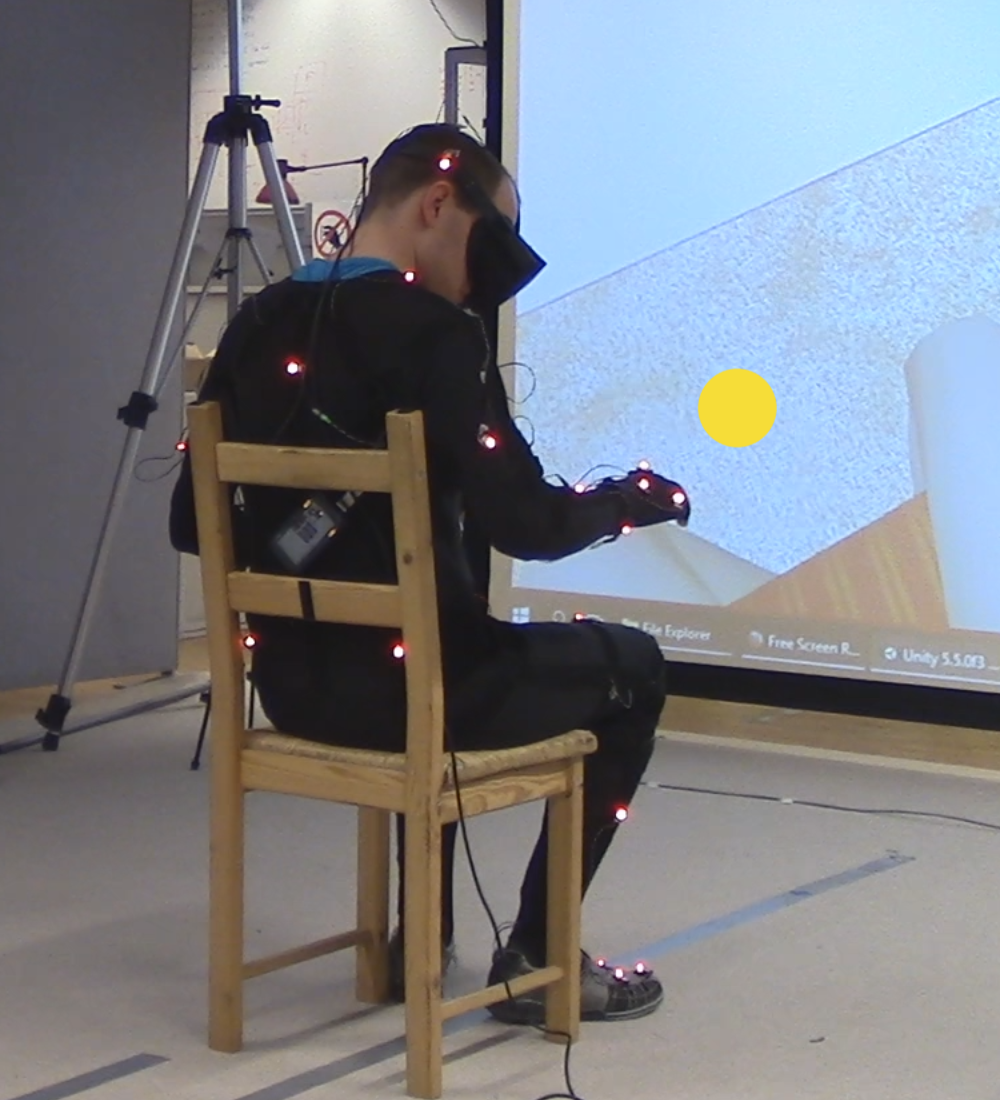
\includegraphics[width=\textwidth]{Figures/handPositionTarget.png}
    \end{subfigure}
        
    \caption{Pictures of a subject, taken from the same point of view, reaching for the same target but with two different distortions of \SI{0}{\decibel} and \SI{3}{\decibel}, with a visual representation of where the target is (yellow dot). The left image shows the \SI{0}{\decibel}, the right one has a distortion of \SI{3}{\decibel}, and the center one is the superimposition of both images.}
    \label{fig:realMocapDistortion}
\end{figure}

This means that in order to perform the same perceived movement, the subject once had to cover the whole distance between his leg and the target, and could in a second time roughly travel two times less in order to reach that target.

\section{Experiment}

---link to the summary video of the experiment---
